\chapter{Demonstrativ- vs. Definitartikel}\label{chap:demdef}

Ein Ziel der vorliegenden Arbeit ist, das funktionale Spektrum von ahd. \object{dër} systematisch zu erfassen und damit die Entwicklung des Definitartikels \is{Definitartikel} im Althochdeutschen nachzuzeichnen. Hierzu sind  Kriterien nötig, die es ermöglichen, De"-mon"-stra"-tiv- von \is{Demonstrativartikel}  Definitartikeln \is{Definitartikel} theoretisch und empirisch voneinander abzugrenzen. In diesem Kapitel wird daher auf Basis der Forschung eine Typologie von definiten Gebrauchskontexten zusammengestellt. Nach einem kurzen Überblick über die wichtigsten Ansätze zur semantischen Analyse definiter Ausdrücke in Abschnitt \ref{sec:definitheitstheorien} führt Abschnitt \ref{sec:demonstrativartikel} in typische Gebrauchskontexte für \isi{Demonstrativartikel}  ein. Davon abgrenzend listet Abschnitt \ref{sec:definitartikel} die Kontexte auf, in denen \isi{Definitartikel} vorkommen. In Abschnitt \ref{sec:pragsem} wird das  Löbnersche Konzept der pragmatischen \is{Pragmatische Definita} und semantischen Definita \is{Semantische Definita} vorgestellt, das sich insbesondere in der historischen Sprachwissenschaft etabliert hat, um Demonstrativ- von Definitartikeln \is{Demonstrativartikel} \is{Definitartikel} zu unterscheiden. 

\section{Semantische Analysen definiter Ausdrücke} \label{sec:definitheitstheorien}

Der \isi{Definitartikel} gilt als prototypischer Ausdruck der grammatischen Kategorie \isi{Definitheit}. Die Frage, was genau unter \isi{Definitheit} zu verstehen ist bzw. welche Funktion dem \isi{Definitartikel} als Vertreter dieser Kategorie innewohnt, ist viel diskutiert und unterschiedlich beantwortet worden \parencite[zum Überblick  s.][]{Bisle-Muller1991,Hauenschild1993,Lyons1999,Abbott2007,Cui2014}.

So ist für die formale Semantik bis heute Russels Einzig"-artig"-keits-Prä"-supposi"-tion (\object{unique"-ness}) relevant, um definite \is{Definitheit} von indefiniten \is{Indefinitheit} Ausdrücken abzugrenzen (vgl. weiterführend \citealt{Russel1905} und \citealt{Heim1991,Heim2011}). Es handelt sich hierbei um einen Beschreibungsansatz, der \is{Nominalphrase (NP)} NPs, die genau einen Referenten denotieren, wie z.B. Unika \is{Unikum} (\object{die Sonne}) oder \is{Superlativ} Superlative (\object{der beste Vortrag}) besonders gut erfassen kann; für  Plural-NPs \is{Nominalphrase (NP)} \is{Numerus} ist er allerdings problematisch \parencite[vgl. die Diskussion hierzu in][7--11] {Lyons1999}. \textcite{Hawkins1978} liefert eine Abwandlung dieses Konzepts: Statt \object{unique"-ness} postuliert er die \object{inclusiveness} definiter Ausdrücke  \parencite[kritisch hierzu:][32]{Bisle-Muller1991}. Dahinter steht die Idee, dass mithilfe des Definitartikels \is{Definitartikel} auf die Gesamtheit aller Referenten, die der definiten Beschreibung genügen, Bezug genommen wird.

Ein weiterer viel zitierter und pragmatisch ausgerichteter Ansatz stammt von \textcite{Christophersen1939}. Demnach können definite NPs \is{Nominalphrase (NP)} nur dann richtig verstanden werden, wenn sowohl der Sprecher als auch der Hörer den Referenten als bekannt einstufen. Diese \object{familiarity}-Theorie kann allerdings allen nicht anaphorisch \is{anaphorisch} gebrauchten Verwendungen des Definitartikels \is{Definitartikel} kaum standhalten wie u.a. \textcite{Hawkins1978} und \textcite{Lobner1985} zeigen. Aufbauend auf \textcite{Lewis1970} versucht \textcite{vonHeusinger1996} den Problemen der traditionellen Definitheitstheorien beizukommen, indem er \isi{Definitheit} mit \object{Salienz} in Verbindung bringt: Definite Ausdrücke beziehen sich demnach immer auf den salientesten Referenten im Diskurs. Dieser Ansatz ist zwar für anaphorische \is{anaphorisch} und situativ-gebrauchte \is{situativ} Definita nützlich, stößt allerdings beim sog. assoziativ-anaphorischen \is{assoziativ-anaphorisch} Gebrauchskontext an Grenzen \parencite[s. auch][144--149]{Cui2014}, da hier der Referent erst über einen Assoziationsprozess aktiviert werden muss und damit gerade keine hohe Salienz aufweist (s. Abschnitt \ref{sec:asso}).

In der historischen Sprachwissenschaft hat sich das Definitheitskonzept von \textcite{Lobner1985} etabliert, um Demonstrativ- \is{Demonstrativartikel} und \isi{Definitartikel} funktional voneinander abzugrenzen \parencite{Demske2001,Szczepaniak2011a,Schlachter2015}. Hierbei wird zwischen pragmatischer \is{Pragmatische Definita} und semantischer Definitheit \is{Semantische Definita} unterschieden; letztere entspricht der Domäne des Definitartikels (vgl. vertiefend Abschnitt \ref{sec:pragsem}). 

Den genannten  semantischen Analysen ist gemein, dass von bestimmten Gebrauchskontexten, die für den \isi{Definitartikel} als typisch angesehen werden, ausgegangen wird \parencite[9]{Cui2014}. Meist steht dahinter das theoretische Ideal, dass sich aus diesen Kontexten \herkur{eine} bestimmte Basisfunktion für den \isi{Definitartikel} erarbeiten lässt. Aus einer historischen Perspektive ist es ganz natürlich, dass eine sprachliche Form unterschiedliche Funktionen übernehmen kann und sich das Verhältnis von Ausdruck und Inhalt über die Zeit wandelt. 

In der vorliegenden Untersuchung geht es um die Frage, welches funktionale Spektrum das ahd. \object{dër} zu bestimmten Zeitpunkten in der Geschichte des Deutschen einnimmt. Konkret soll ermittelt werden, ob \object{dër} in den unterschiedlichen ahd. Überlieferungen als Demonstrativ- \is{Demonstrativartikel} oder \isi{Definitartikel} zu klassifizieren ist. Für die Beantwortung dieser Frage kann man sich die Gebrauchskontexte \is{Definitheitskontext} zunutze machen, die den beiden Artikeltypen in der Forschung zugesprochen werden. Sie sind Gegenstand der nächsten beiden Abschnitte. 


\section{Gebrauchskontexte für Demonstrativartikel}\label{sec:demonstrativartikel}

In allen Sprachen der Welt gibt es Demonstrativa, d.h. deiktische Ausdrücke, die auf außersprachliche Entitäten verweisen oder diskursintern Wissen (re)ak"-ti"-vieren \parencite{Diessel1999, Diessel2006}. Neben pronominalen (\object{Wusstest du das?}) und adverbial gebrauchten Demonstrativa \is{Demonstrativum} \is{Adverbial} (z.B. \object{hier}) unterscheidet man die Klasse der adnominalen \is{Demonstrativum} Demonstrativa, also der \isi{Demonstrativartikel} (\object{Ich kaufe mir dieses/jenes Buch}), aus denen  \isi{Definitartikel} typischerweise hervorgehen (s. ausführlich Kapitel \ref{chapter:theorie}). Es werden vier Kontexte unterschieden, in denen \isi{Demonstrativartikel} auftreten: der \is{situativ} situative, der \is{anaphorisch} anaphorische, der diskursdeiktische \is{diskursdeiktisch} und der anamnestische \is{anamnestisch} Gebrauchskontext \parencite[s. u.a.][]{Hawkins1978,Lyons1979,Bisle-Muller1991,Himmelmann1996,Himmelmann1997,Fillmore1997,Diessel1999,Schwarz2000,Consten2004,Diessel2006,Diessel2012, Studler2011}. Diese lassen sich anknüpfend an die Terminologie von \textcite{Halliday1993} unter die Begriffspaare exophorisch (=\,situativ) und endophorisch (= nicht-situativ) fassen \parencite[vgl. auch][6]{Diessel1999}; zur Übersicht s. Abbildung~\ref{abb:demonstrativa-gebrauchskontexte}. Für die Entwicklung des Definitartikels sind die endophorischen Kontexte (vor allem der anaphorische \is{anaphorisch} und der anamnestische \is{anamnestisch} Gebrauch) besonders relevant, da sie kategorielle Schnittstellen zum \isi{Definitartikel} bilden (vgl. ausführlich die Diskussion in \ref{sec:bruecke}). In den nachfolgenden Abschnitten erfolgt die Erläuterung der einzelnen Kontexte.

\begin{figure}[h]
% 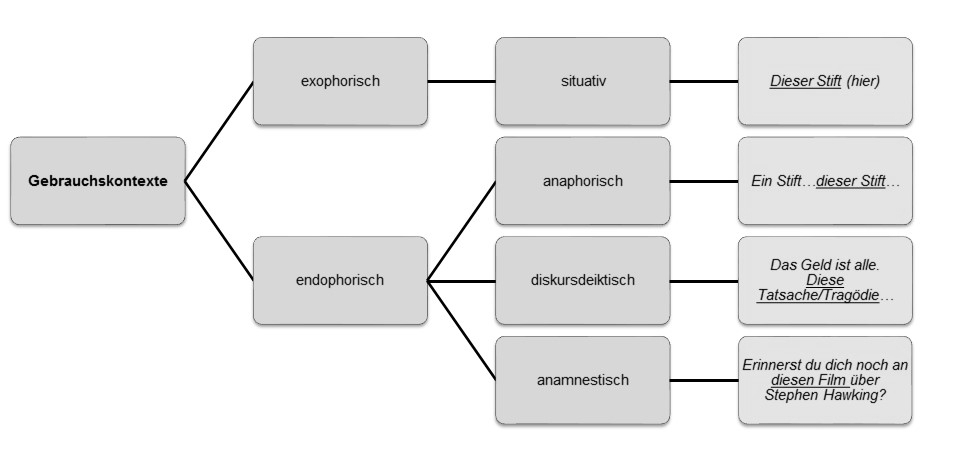
\includegraphics[width=12cm]{images/Gebrauchskontexte-demonstrativa-neu-sw.jpg}
\begin{forest}
for tree = {forked edges,grow'=east,anchor=east,minimum width=2cm,align=center,draw,s sep=\baselineskip}
[Gebrauchskontexte,rotate=90,anchor=north
  [exophorisch [ situativ,tier=isch [ \textit{Dieser Stift} (hier) ] ] ]
  [endophorisch
    [anaphorisch,tier=isch [ Ein Stift\ldots\textit{dieser Stift}\ldots ] ]
    [diskursdeiktisch,tier=isch [Das Zahlen steigen.\\\textit{Diese Entwicklung} ist\ldots ] ]
    [anamnestisch,tier=isch [ Erinnerst du dich noch\\an \textit{diesen Film} über\\Stephen Hawking? ] ]
  ]
]
\end{forest}
\caption {Gebrauchskontexte von Demonstrativa\label{abb:demonstrativa-gebrauchskontexte}}
\end{figure}



\subsection{Situativer Gebrauch}\label{sec:situativ}

Beim situativen \is{situativ} Gebrauch \parencite[auch deiktischer Gebrauch, z.B. bei][]{Bisle-Muller1991,Consten2004,Studler2011} führt der \isi{Demonstrativartikel} einen Referenten in das gemeinsame Diskursuniversum von Sprecher und Hörer ein, indem mit seiner Hilfe auf eine Entität in der unmittelbaren Äußerungssituation verwiesen wird, s. \REF{ex:deikt}.\footnote{In diesem und den folgenden Beispielen werden die relevanten Ausdrücke durch Kursivsetzung durch die Verfasserin hervorgehoben.}  Zugleich erfolgt eine Verortung im Raum.

\begin{exe}
	\ex \label{ex:deikt} \object{Dieser Stift} (hier) schreibt gut.
\end{exe}

Proximale Demonstrativa \is{Demonstrativum} kennzeichnen Entitäten, die dem Sprecher nahe\linebreak sind (z.B. \object{dieser}), distale markieren Distanz (z.B. \object{jener, dieser/der da}).
%\footnote{Diese Zweigliedrigkeit ist in allen Sprachen der Welt gegeben; zu komplexeren Systemen s. \textcite[35--55]{Diessel1999}.} 
Damit das Referieren glückt, müssen die Diskursteilnehmer ihr Wissen mit der Perspektive des Sprechers, dem deiktischen Zentrum oder  \object{origo} \parencite{Buhler1934} abgleichen  \parencite[s. auch][327--330]{Hoffmann2009}. Der Verweis kann mit einer Zeigegeste unterstützt werden; zu Ausnahmen und weniger zentralen Fällen des situativen \is{situativ} Gebrauchs s. \textcite[94--95]{Diessel1999} und \textcite[219--224]{Himmelmann1996}. 

Mit \textcite[]{Buhler1934} kann man den situativen \is{situativ} Gebrauch in zwei Arten des Zeigens unterteilen. Bei der sog. \object{Demonstratio ad oculos} zielt die Zeigegeste auf einen Referenten, der in der unmittelbaren Umgebung vorhanden und somit für die Diskursteilnehmer sichtbar ist (typisch für \object{Face-to-Face}-Kommunikation). Die sog. \object{Deixis am Phantasma} umfasst hingegen demonstrative Ausdrücke, die innerhalb der bloßen Vorstellung operieren: Der Referent wird zwar im Diskursuniversum verortet, ist aber nicht physisch anwesend \parencite[s. auch][222]{Himmelmann1996}. Dieser Gebrauch gilt für alle Kommunikationsformen, in denen Äußerungen zeitlich und räumlich vom Sprecher entkoppelt sind, also z.B. in narrativen Texten \parencite[95]{Diessel1999} oder auch in wissenschaftlichen Beschreibungen, in denen das deiktische Zentrum von einem imaginären Sprecher ausgeht. Der situative \is{situativ} Gebrauch ist in diesem Sinne auch in Dokumenten aus älteren Sprachstufen zu erwarten. 

Mit der situativen \is{situativ} Verortung -- sei sie konkret oder imaginär -- geht immer ein kognitiver Abgrenzungsprozess zu anderen potentiellen Referenten einher, etwa  \object{Ich möchte diesen (und nicht jenen) Stift} \parencite[vgl.][70]{Bisle-Muller1991}, wodurch der Referent eindeutig determiniert und identifiziert werden kann \parencite{Hoffmann2009}. 

 
\subsection{Anaphorischer Gebrauch}\label{sec:anaphorisch}

Während die eindeutige Determination beim situativen \is{situativ} Gebrauch über den außersprachlichen Kontext gewährleistet wird, kommt beim anaphorischen \is{anaphorisch} Ge"-brauch die textuelle Umgebung ins Spiel\footnote{Die textuelle Umgebung schließt sowohl schriftliche als auch mündlich Diskurstypen ein.}: Es wird auf einen zuvor im Diskurs etablierten Referenten verwiesen (den Antezedens), s. \REF{ex:anaph} basierend auf \textcite[][229]{Himmelmann1996}.{\interfootnotelinepenalty=10000\footnote{In Opposition hierzu stehen \object{kataphorische} Ausdrücke: Sie sind koreferentiell \is{Referentialität} mit nachfolgenden Referenten, welche erst im weiteren Diskursverlauf  hinreichend identifiziert werden können \parencite[s.][161--162]{Veldre-Gerner2007}. Beim vergleichsweise seltenen kataphorisch gebrauchten \isi{Demonstrativartikel} kann eine pejorative Lesart mitschwingen (\object{Auf der Party war dieser Student. Er hieß John und...}). Zur Diskussion solcher Verwendungsweisen als möglichen Ausdruck von \isi{Spezifizität} s. \textcite[533]{deMulder2011}.}}

\begin{exe}
	\ex \label{ex:anaph} Es war einmal ein König. \object{Dieser König} hatte drei Söhne...
\end{exe}

Im Vergleich zu anderen Mitteln der Wiederaufnahme \is{Personalpronomen}  (etwa Personalpronomen\linebreak oder \isi{Definitartikel}) zeichnen sich anaphorische \is{anaphorisch} \isi{Demonstrativartikel} (und Demonstrativa \is{Demonstrativum} allgemein) dadurch aus, dass sie eine (Neu-)Fokussierung von Referenten im Diskurs bewirken \parencite [s. u.a.][]{Ehlich1979,Prince1981,Gundel1993,Comrie1997,Himmelmann1996,Diessel1999,Kibrik2011}. Sie werden daher häufig gebraucht, um einen Topikwechsel \is{Topik} \isi{Informationsstruktur} zu vollziehen. In Beispiel \REF{ex:topic} \parencite[angelehnt an][96]{Diessel1999}, impliziert das \isi{Personalpronomen} \object{er} Koreferentialität \is{Referentialität} mit dem \isi{Topik} \object{Anwalt}, während sich das \isi{Demonstrativum} \object{der} nur auf \object{Klient} beziehen kann, der zu diesem Zeitpunkt zwar kognitiv aktiviert, aber nicht fokussiert und \blockcquote[96]{Diessel1999}{somewhat unexpected} ist \parencite[vgl. hierzu][278--279]{Gundel1993}. Im Gegensatz hierzu ist die Wiederaufnahme des bereits im Fokus stehenden \object{Anwalt} mit \object{dieser Anwalt} blockiert. Am natürlichsten erscheinen die pronominalen \isi{Informationsstruktur} Wiederaufnahmen. Mit der \isi{Phrase} \object{dieser Klient} kann allerdings besonders stark betont werden, dass jetzt der Klient und nicht -- wie erwartet -- der Anwalt im Mittelpunkt des weiteren Diskursverlaufs steht.   

\begin{exe}
	\ex \label{ex:topic} Der Anwalt sprach mit einem Klienten. Da \object{er/der/dieser Klient/*dieser Anwalt} nur wenig Zeit hatte, vereinbarten sie ein weiteres Gespräch für die nächste Woche. 
\end{exe}

Das Potential, einen Topikwechsel \is{Topik} einzuleiten, lässt sich darauf zurückführen, dass es zur Hauptfunktion von Demonstrativa \is{Demonstrativum} gehört, Referenten, die gerade neu eingeführt wurden, anaphorisch \is{anaphorisch} wiederaufzunehmen.\footnote{Vgl. hierzu auch die Studie von \citeauthor{Fraurud1990}, in der empirisch belegt wird, dass schwedische \isi{Demonstrativartikel} fast ausschließlich anaphorisch \is{anaphorisch} gebraucht werden \parencite[400]{Fraurud1990}.} Dies gilt insbesondere für artikellose Sprachen  \parencite[229]{Himmelmann1996}, aber auch für Sprachen, die einen \isi{Definitartikel} ausgebildet haben, etwa das Englische. \citeauthor{Christophersen1939} beobachtet \blockcquote[vgl.][29]{Christophersen1939} {a certain aversion to the use of a \object{the}-form immediately after the word is introduced; a demonstrative is more usual in such cases}. Demonstrativa \is{Demonstrativum} sind also die erste Wahl, um ein \isi{Topik} im Diskurs nach Ersterwähnung des Referenten zu etablieren. Für die  anschließende referentielle Kontinuität \is{Informationsstruktur} sorgen \isi{Personalpronomen} oder \isi{Definitartikel}, indem sie das \isi{Topik} im Fokus der Aufmerksamkeit halten. 

\subsection{Diskursdeiktischer Gebrauch}\label{diskurs-deikt}

Werden \isi{Demonstrativartikel} zum Zwecke der Diskursdeixis \is{diskursdeiktisch} eingesetzt, verweisen sie nicht auf einzelne \is{Nominalphrase (NP)} NPs, sondern auf größere syntaktische Einheiten, also Sätze, Abschnitte oder Texte \parencite{Webber1991,Fraurud1992, Fillmore1997, Diessel1999, Consten2007, Consten2009, Marx2011}. Durch die anaphorische \is{anaphorisch} Wiederaufnahme werden die zuvor genannten Informationen zu einem abstrakten Referenten gebündelt (z.B. \object{Tatsache, Prozess, Zustand}) und können dann evaluierende Zusatzinformationen transportieren (\object{Ungerechtigkeit, Tragödie, Zufall}),  s. (\ref{diskurs}).\footnote{Da dieser anaphorische \is{anaphorisch} Prozess die \blockcquote[129]{Schwarz2000}{kognitive Strategie der Komplexbildung} voraussetzt, hat sich in neueren Arbeiten zur Textlinguistik der Begriff \object{Komplex-Anaphern} etabliert \parencite[s. z.b.][]{Consten2007, Consten2009}. Einen Überblick über weitere terminologische Vorschläge der letzten Jahrzehnte bietet \textcite[16--17]{Marx2011}, zur Abgrenzung von Diskursdeixis \is{diskursdeiktisch} und Anapher \is{anaphorisch} s. \textcite[30--31]{Consten2004}.} 

 \begin{exe}
	\ex \label{diskurs}  Jedes Jahr sind tausende Menschen auf der Flucht.
	\begin{xlist}
		\ex \label{propo} \object{Diese Tatsache} lässt viele erschauern.
			\ex \label{bewertung} \object{Diese Ungerechtigkeit} muss behoben werden.
		\end{xlist}
\end{exe}

Zwar kann der diskursdeiktische Gebrauch nur über einen anaphorischen \is{anaphorisch} Bezug gelingen, der eigentliche Referent wird allerdings erst zum Zeitpunkt des Verweises im Diskurs etabliert, wodurch die Diskursdeixis dem situativen \is{situativ} Gebrauchskontext ähnelt \parencite[224]{Himmelmann1996}. Beide Kontexte fallen typischerweise in die Domäne von pro- oder adnominalen Demonstrativa; ein Austausch mit dem \isi{Definitartikel} ist theoretisch möglich, aber markiert, vgl. (\ref{def-diskurs}); Beispiele nach  \textcite[130--131]{Schwarz2000}.  

 \begin{exe}
	\ex \label{def-diskurs} 
	\begin{xlist}
		\ex \label{ex:tassen} Er zerbrach bei der Feier eine sehr teure Vase. \object{Dieses/Das Missgeschick} blieb noch lange in Erinnerung. 
			\ex \label{ex:entwicklung} Die Arbeitslosigkeit steigt, die Inflation schreitet fort, die Wirtschaft ist rückläufig. \textit{Diese/}??\textit{Die Entwicklung} ist gefährlich. 
		\end{xlist}
\end{exe}

Die Faktoren, die bestimmen, dass NPs \is{Nominalphrase (NP)} mit \isi{Definitartikel} für den diskursdeiktischen \is{diskursdeiktisch} Gebrauch gewählt werden, sind bislang kaum erforscht. Mit der Korpusuntersuchung \is{Korpuslinguistik} von \textcite{Consten2007} ist allerdings empirisch belegt, dass \isi{Demonstrativartikel} das häufigste und damit unmarkierte Mittel sind, um im Deutschen diskursdeiktische \is{diskursdeiktisch} Bezüge herzustellen.

\subsection{Anamnestischer Gebrauch}\label{sec:amnamnestisch}

Beispiel \REF{ex:anamn} illustriert den anamnestischen \is{anamnestisch} Gebrauchskontext. Der Referent von  \object{dieser Aufsatz} wird als neue Information \is{Informationsstruktur} in den Diskurs eingeführt. Für die eindeutige Identifizierung muss der Rezipient allerdings vorhandenes Wissen aktivieren, d.h. Informationen, die im Langzeitgedächtnis gespeichert sind.

\begin{exe}
	\ex \label{ex:anamn} Hast du schon \object{diesen Aufsatz} von der neuen Kollegin gelesen?  
\end{exe}

Der Begriff \object{anamnestisch} \is{anamnestisch} geht auf \textcite{Buhler1934} zurück (von griech. \object{anámnesis} \extrans{Erinnerung}) und wurde von \textcite{Himmelmann1997} als deutsche Übersetzung des \object{recognitional use} \parencite{Himmelmann1996,Diessel1999}  eingeführt.

Die Voraussetzung für diesen Gebrauchskontext ist, dass die Diskursteilnehmer gleiche Erfahrungen über den gemeinten Referenten besitzen, etwa durch ein früheres Gespräch. \textcite[44]{Bisle-Muller1991} spricht in diesem Sinne von \object{konspirativem Wissen}; auch engl. \object{private information} \parencite[106]{Diessel1999}. Die Identifizierbarkeit des Referenten ist daher an die notwendige Mitwisserschaft des Hörers gekoppelt \parencite[72]{Szczepaniak2011a}. Für den Sprecher sind anamnestische \is{anamnestisch} Verweise besonders ökonomisch, da der Appell zur gemeinsamen Wissensaktivierung mit vergleichsweise geringen verbalen Kosten verbunden ist. Für den Hörer ist der (kognitive) Erinnerungsaufwand umso größer.

Nach \textcite[79--80]{Bisle-Muller1991} kann die Verwendung des Demonstrativartikels \is{Demonstrativartikel} in diesen Kontexten sogar als kommunikative Strategie genutzt werden, um eine mögliche Uneindeutigkeit des Referenten zu kennzeichnen, s. \REF{ex:auer} (Gesprächsbeispiel vereinfacht nach \citealt[637]{Auer1984}, vgl. auch \citealt[58]{Himmelmann1997}). Der Sprech"-er räumt sozusagen die Möglichkeit ein, dass es dem Hörer Schwierigkeiten bereiten könnte, einen eindeutigen Referenten für die Phrase \is{Phrase} \object{diesem Haustelefon} auszumachen. 

\begin{exe}
	\ex \label{ex:auer} 
	\begin{itemize}
		\item[A:] Was ist denn eigentlich mit \textit{diesem Haustelefon}, das ihr immer genutzt habt? 
		\item[B:] Das funktioniert nicht mehr. 
	\end{itemize}
\end{exe}

Die mögliche Referenzproblematisierung durch \object{dieser} schwingt beim \isi{Definitartikel} nicht mit, vgl. Beispiel \REF{ex:kinder} \parencites()()[][80]{Bisle-Muller1991}[][70]{Himmelmann1997}. Wenn von \object{den Kindern} gesprochen wird, ist die naheliegendste Interpretation, dass die eigenen Kinder gemeint sind; mit \object{diese Kinder} wird ein breiterer (und unerwarteter) Wissensrahmen eröffnet, der nur mit Bezug auf geteiltes Wissen eine eindeutige Referenz zulässt.    

\begin{exe}
	\ex \label{ex:kinder} Ich bringe heute \textit{die Kinder/diese Kinder} mit.   
\end{exe}

Der anamnestische \is{anamnestisch} wird neben dem anaphorischen \is{anaphorisch} Gebrauch als möglicher Übergangsbereich von Demonstrativ- zu \isi{Definitartikel} betrachtet (s. ausführlich die Diskussion in Abschnitt \ref{sec:bruecke}). Laut \textcite[73]{Himmelmann1997} sind für den anamne"-stischen Gebrauch \object{aktivierende Modifikatoren} typisch. Hierzu zählen bspw. das PP-Attribut \object{von der neuen Kollegin} aus Beispiel \REF{ex:anamn} oder restriktive Relativsätze wie in dem nachfolgenden Beispiel.

\begin{exe}
	\ex \label{ex:film} Sie geht in \textit{diese neue Schule, auf der man nicht sitzenbleiben kann}.    
\end{exe}
\noindent 
Die Beschreibung im Relativsatz soll dem Hörer oder der Hörerin helfen, sich den Referenten in Erinnerung zu rufen. Es wird vorausgesetzt, dass dem Adressaten die Schule (z.B. durch vorherige Gespräche) bekannt ist. Im Unterschied zu den \object{etablierenden Modifikatoren} (s. Abschnitt \ref{sec:nicht-fam}) nimmt die Identifikationshilfe im Relativsatz Bezug auf Wissen, das nur von den Diskursteilnehmern geteilt wird. Durch etablierende Modifikatoren wird ein Referent hingegen durch Einbezug von generellerem Wissen definiert und damit eindeutig identifiziert, etwa \object{Sie freut sich auf das Buch von George R.R. Martin, das morgen erscheint}. Weil die Grenze zwischen diesen beiden Modifikationsarten fließend sind, sind Brückenkontexte \is{Brückenkontext} hier wahrscheinlich \parencite[s. zur ausführlichen Diskussion][79--80]{Himmelmann1997}. 

\section{Gebrauchskontexte für Definitartikel}\label{sec:definitartikel}

Wie nachfolgend gezeigt wird, kann der \isi{Definitartikel} prinzipiell auch in den für das \isi{Demonstrativum} typischen Verwendungsweisen vorkommen, die in den vorhergehenden Abschnitten erläutert wurden (Abschnitt \ref{sec:definitartikel-in-demonstrativ}). Darüber hinaus gibt es Gebrauchskontexte, die alleine den Definitartikeln vorbehalten sind. Hierzu zählen der abstrakt-situative Gebrauch \is{abstrakt-situativ} (Abschnitt \ref{sec:abst-sit}), der assoziativ-anaphorische \is{assoziativ-anaphorisch} Gebrauch (\ref{sec:asso}), die sog. nicht-familiären (\ref{sec:nicht-fam}) und die nicht-referentiellen \is{Referentialität} Gebrauchs"-kontexte (Abschnitt\ref{sec:nicht-referentiell}). 

\subsection{Verwendung in demonstrativen Gebrauchskontexten}\label{sec:definitartikel-in-demonstrativ}

Belege für den situativen \is{situativ} und anaphorischen \is{anaphorisch} Gebrauch finden sich bei \textcite[110--111]{Hawkins1978} und \textcite[36]{Himmelmann1997}, s. \REF{ex:sitdef} und \REF{ex:anadef}; nachfolgend übersetzt und leicht gekürzt.\footnote{In der Forschung wird für die Kontextanalysen meist das Englische als Bezugssprache genommen \parencite{Christophersen1939, Lobner1985,Lyons1999}. Typologische Vergleiche finden sich in \textcite{Himmelmann1997}, für das Deutsche sei auf \textcite{Bisle-Muller1991} verwiesen.} Die Bedeutungsunterschiede sind in diesen Beispielen minimal: Beim \isi{Demonstrativum} schwingt aufgrund seiner deiktischen Kraft ein Abgrenzungsmoment zu anderen (wenn auch nicht explizit genannten) Referenten mit \parencite{Bisle-Muller1991}; außerdem hebt es den Topikwechsel \is{Topik} hervor.\footnote{Mit Akzentuierung (\object{dér}) kann auch der \isi{Definitartikel} in dieser Form verwendet werden.}   

\begin{exe}
	\ex \label{ex:sitdef} Reich mir bitte mal \textit{diesen/den Eimer}.  \\(situativer \is{situativ} Gebrauch)
	\ex \label{ex:anadef} Ein Mann erscheint mit einem Paket. Und \textit{dieses/das Paket}... \\(anaphorischer Gebrauch)
\end{exe}

Anders sieht es beim diskursdeiktischen \is{diskursdeiktisch} Gebrauch aus. Hier ist die Substitution mit einem \isi{Definitartikel} ebenfalls möglich, aber deutlich markiert, s. \REF{ex:diskurs-deikt-def}; Beispiel aus \textcite[95]{Marx2011}, vgl. auch Abschnitt \ref{diskurs-deikt}). Während die Phrase \is{Phrase} \object{diese Nachlässigkeit} den Zustand, den man aus dem vorher genannten Ereignis ableiten kann, klassifiziert und damit indirekt anaphorisch  \is{anaphorisch} ist, kann \object{die Nachlässigkeit} als allgemeine Last interpretiert werden, die \object{Robert} auszeichnet, im Sinne von \object{seine Nachlässigkeit}.

\begin{exe}
	\ex \label{ex:diskurs-deikt-def}  Anstatt für seine Prüfungen zu lernen, ist Robert im Kino gewesen. \textit{Diese\slash}?\textit{Die Nachlässigkeit} könnte ihn das Vordiplom kosten. \\(diskursdeiktischer Gebrauch)
	 \end{exe}

Auch beim anamnestischen \is{anamnestisch} Gebrauch kommt es zu Bedeutungsunterschieden, s. \REF{ex:anamndef}. Mit dem \isi{Definitartikel} unterstellt der Sprecher,  dass der Referent mit Rückbezug auf geteiltes Wissen problemlos identifiziert werden kann; die Phrase \is{Phrase} mit \isi{Demonstrativartikel} signalisiert hingegen, dass es möglicherweise nicht direkt klar ist, welcher Wissensrahmen aktiviert werden muss, um den Referenten zu verorten \parencite[79--80]{Bisle-Muller1991}. 
 
\begin{exe}
	\ex \label{ex:anamndef} Ich habe doch noch \textit{dieses/das Buch} gekauft. \\ (anamnestischer Gebrauch)
\end{exe}
 
Während in den nhd. Beispielen jeweils zwei Formen kontrastiert wurden (De"-mon"-strativ"-artikel \is{Demonstrativartikel} \object{dieser} vs. \isi{Definitartikel} \object{der}), gibt es im Althochdeutschen \object{eine} Form, die sowohl De"-mon"-strativ-"" \is{Demonstrativartikel} als auch \isi{Definitartikel} sein könnte, nämlich das ahd. \object{dër}. 
Wenn ein \object{dër}  in den bisher genannten Verwendungsweisen, den sog. pragmatischen \is{Pragmatische Definita} Definitheitskontexten (s. Abschnitt \ref{sec:pragsem}) genutzt wird, so kann man es folglich immer als Demonstrativartikel, aber nicht automatisch als \isi{Definitartikel} einordnen. Allgemeiner formuliert: Kommt ein Artikelwort in pragmatischen Definitheitskontexten \is{Pragmatische Definita} vor, ist dies keine  hinreichende Bedingung dafür, dass es sich um einen Definitartikel-, wohl aber um einen \isi{Demonstrativartikel} handelt. Wenn ein Artikelwort aber in den sog. semantischen Definitheitskontexten \is{Semantische Definita} auftritt, betritt es die Domäne des Definitartikels. Zu diesen zählen die abstrakt-situativen \is{abstrakt-situativ} und die assoziativ-anaphorischen \is{assoziativ-anaphorisch} Gebrauchskontexte, die in den folgenden Abschnitten besprochen werden. 



\subsection{Abstrakt-situativer Gebrauch}\label{sec:abst-sit}

Abstrakt-situative \is{abstrakt-situativ} Gebrauchskontexte zeichnen sich dadurch aus, dass ein Referent auch unabhängig von der Gesprächssituation eindeutig bestimmt werden kann \parencite[daher auch \object{larger situation use}, vgl.][115]{Hawkins1978}. Der  Referent ist also nicht in deiktischer inner- oder außersprachlicher Reichweite, sondern wird über das Weltwissen erschlossen. Dabei kann der jeweilige Wissensrahmen, in dem der Referent verortet wird, variieren. Die definiten NPs \is{Nominalphrase (NP)} in \REF{ex:abstrakt-situativ} basieren bspw. auf der Erfahrung, dass eine Stadt typischerweise \object{ein} Rathaus (\ref{ex:rathaus}),  Deutschland \object{eine}  Bundeskanzlerin (\ref{ex:merkel})  und unsere Erde \object{einen} Mond (\ref{ex:mond}) hat. Die Beispiele setzen also voraus, dass die Referenten \is{abstrakt-situativ} in einem bestimmten Bezugsrahmen \object{einzigartig} \parencite{Russell2006} sind. 

 \begin{exe}
	\ex \label{ex:abstrakt-situativ}   
	\begin{xlist}
		\ex \label{ex:rathaus} Wir treffen uns vor \textit{dem Rathaus}.
		\ex \label{ex:merkel} \textit{Die Bundeskanzlerin} kommt zu Besuch.
		\ex \label{ex:mond} Gestern schien \textit{der Mond} besonders hell.
		\end{xlist}
\end{exe}

Wichtig ist, dass die Diskursteilnehmer denselben Bezugsrahmen aktivieren. Beispielsweise gibt es theoretisch unendlich viele Personen, auf die mit \object{der Bräutigam} in \REF{ex:braut} referiert werden kann, aber innerhalb eines spezifischen situativen Rahmens (hier das Gespräch über eine bestimmte Hochzeit, auf der es dem Weltwissen nach zu urteilen typischerweise einen Bräutigam gibt), können die Diskursteilnehmer präsupponieren, dass die Referenz eindeutig ist \parencite[Beispiel in Adaption an][41]{Studler2011}. Ebenso ist für Diskursteilnehmer \object{die Kneipe} in \REF{ex:kneipe} eindeutig identifizierbar, wenn es um die Kneipe geht, in der man sich regelmäßig trifft \parencite[36]{Himmelmann1997}.

\begin{exe}
	\ex \label{ex:abstrakt-situativ2}   
	\begin{xlist}
		\ex \label{ex:braut} Kanntest du \textit{den Bräutigam} gut?
		\ex \label{ex:kneipe} Wir treffen uns in \textit{der Kneipe}.  
		\end{xlist}
\end{exe}

Ein \isi{Unikum} wie \object{der Mond} ist hingegen weitaus weniger kontextsensitiv; seine Identifizierbarkeit ist fast in jedem Gespräch und zu jeder Zeit gesichert \parencite[549]{Schroeder2006}. \textcite[40--41]{Studler2011} folgend lässt sich die abstrakt-situative \is{abstrakt-situativ} Verwendungsweise von Definitartikeln \is{Definitartikel} daher aufteilen in \object{absolut-uniken} (bei\linebreak Unika) \is{Unikum} und \object{situativ-uniken} Gebrauch (wie in \ref{ex:braut}). In beiden Kontexten ist der Austausch mit einem \isi{Demonstrativartikel} nicht möglich. 

Nach \citeauthor{Schroeder2006} zählt auch der Verweis auf Institutionen wie in \REF{ex:post} zum abstrakt-situativen \is{abstrakt-situativ} Gebrauchskontext \parencite[vgl. auch][110]{Nubling2005}:  \blockcquote[549]{Schroeder2006}{As an institution, \object{the post office} may refer uniquely, even if I and the person I am speaking to merely share the context of living in a country with an institutionalized postal service}. 

\begin{exe}
	\ex \label{ex:post} Ich gehe \textit{zur Post}.
\end{exe}

\noindent
Die Beispiele in \REF{ex:rathaus} und \REF{ex:kneipe} können ebenfalls eine solche Institutionslesart haben. Weil kein spezifischer Referent denotiert wird, ergibt sich in diesen Fällen eine konzeptuelle Nähe zu nicht-spezifischen \is{Spezifizität}
 Gebrauchskontexten, s. Abschnitt \ref{sec:nicht-referentiell}.

Abstrakt-situative \is{abstrakt-situativ} Verwendungen weisen zudem Überschneidungspunkte mit dem anamnestischen \is{anamnestisch} Gebrauch auf \parencite[62]{Himmelmann1997}. In beiden Fällen wird erst über die Aktivierung von gemeinsamem Wissen ein Rahmen geschaffen, der die Identifizierbarkeit eines Referenten ermöglicht. Der Unterschied liegt darin, dass es sich bei der anamnestischen \is{anamnestisch} Verwendung um für die Diskursteilnehmer exklusives und auf spezifische Erfahrungen basiertes Wissen handelt, während der abstrakt-situative \is{abstrakt-situativ} Gebrauch auf Erfahrungen basiert, die ins Allgemeinwissen übergegangen sind. 

\subsection{Assoziativ-anaphorischer Gebrauch}\label{sec:asso}

Der assoziativ-anaphorische \is{assoziativ-anaphorisch} Artikelgebrauch liegt vor, wenn sich die definite Referenz aus einem Assoziationsverhältnis ergibt, das durch einen vorhergehenden Ausdruck im Text -- dem \object{trigger} \parencite[49]{Hawkins1978} oder \object{Anker} \parencite[6]{Cui2014} -- ausgelöst wird. So ist der \object{Kellner} in \REF{ex:asso} über eine Assoziationskette mental aktiviert, wenn über einen Restaurantbesuch gesprochen wird \parencite[Beispiel in Anlehnung an][50]{Schwarz2000}. Neben dem Terminus \is{assoziativ-anaphorisch} \object{assoziativ-anaphorisch}, der auf die Definitartikel-Typologie von \textcite{Hawkins1978} zurückgeht, werden in der Forschung u.a. die Begriffe  \object{bridging} \parencite{Clark1977}, \object{inferables} \parencite{Prince1981} oder \object{indirekte Anaphorik} \parencite{Schwarz2000} für diesen Gebrauchskontext verwendet.  

\begin{exe}
	\ex \label{ex:asso} Wir besuchten gestern ein Restaurant. [Anker] \\ 
	\textit{Der Kellner} [= assoziativ-anaphorische \is{assoziativ-anaphorisch} NP] war sehr nett zu uns. \end{exe}
\noindent 
Wichtig ist, dass das Bezugselement und der daran anknüpfende definite Ausdruck in einer \blockcquote[36]{Himmelmann1997}{kulturell oder sachlich vermittelten} Assoziationsrelation stehen, ansonsten ist die Textkohärenz gestört, s. \REF{ex:hund} im Vergleich zu \REF{ex:auspuff}; die Bespiele basieren auf \textcite[123]{Hawkins1978}.

 \begin{exe}
	\ex \label{ex:asso2}   
	\begin{xlist}
		\ex \label{ex:auspuff} Ein Auto fuhr an uns vorbei. \textit{Der Auspuff} stank. 
		\ex \label{ex:hund} Ein Auto fuhr an uns vorbei. \textit{Der Hund} bellte.
		\end{xlist}
\end{exe}

Mentale Assoziationsketten können also auf Teil-Ganzes-Re"-la"-tio"-nen beruhen (ein Auspuff ist ein typischer Bestandteil von Autos, ein Hund nicht), s. auch \REF{ex:meronymie}. Weitere Typen der \object{Verankerung} erörtert \textcite[98--122]{Schwarz2000}: Der semantische Valenzrahmen von Verben eröffnet bspw. Leerstellen für Partizipantenrollen, \is{Semantische Rolle} die als Bezugspunkt für assoziative Anaphern dienen können, s. \REF{ex:rolle}. Ein nominaler Ausdruck wie \object{das Krankenhaus} aktiviert ein kognitives \isi{Schema} mit bestimmten Standardwerten (etwa \object{Ärzte, Personal, Zimmer}), auf die indirekt verwiesen werden kann, s. \REF{ex:krank}. 

\begin{exe}
	\ex \label{ex:asso3}   
	\begin{xlist}
		\ex \label{ex:meronymie} Dort steht ein \is{Metonymie} Haus. \\ \textit{Das Fenster/die Tür/der Balkon} ist blau gestrichen. (Teil-Gan"-zes-Re"-la"-tion)
		\ex \label{ex:rolle} Heute wurde über eine Entführung berichtet. \\ \textit{Die Kidnapper} (=\,Agensrolle \isi{Agentivität} von \object{entführen}) fordern ein hohes Lösegeld.
				\ex \label{ex:krank} Sie musste ins Krankenhaus. \\ \textit{Die Ärzte/die Pfleger/das Wartezimmer}...\\(Standard-Werte für das Krankenhaus-Schema)
		\end{xlist}
\end{exe}

Ähnlich wie beim abstrakt-situativen \is{abstrakt-situativ} Gebrauchskontext wird enzyklopädisches Wissen bzw. auf Erfahrungen basierendes Weltwissen \hervor{angezapft}, das unabhängig von der Äußerungssituation für die notwendige Identifizierbarkeit des Referenten sorgt. Der Austausch mit einem \isi{Demonstrativartikel} ist in diesen Fällen entweder nicht möglich oder mit einer Bedeutungsverschiebung verbunden, z.B. mit einem pejorativen Unterton \parencite[989]{Hauenschild1993}. Wenn ein adnominales Element regelmäßig in abstrakt-situativen \is{abstrakt-situativ} und assoziativ-anaphorischen \is{assoziativ-anaphorisch} Kontexten verwendet wird, ist daher eine Einordnung als \isi{Definitartikel} gerechtfertigt \parencite[190]{Himmelmann1997}.

\subsection{Nicht-familiärer Gebrauch}\label{sec:nicht-fam}

\textcite[130--149]{Hawkins1978} führt unter den sog. \object{unfamiliar usages} unterschiedliche Gebrauchs"-typen an, in denen der \isi{Definitartikel} im Englischen gesetzt wird. Sie wurden von ihm als Gegenbeispiele für \citeauthor{Christophersen1939}s \object{familiarity}-Theorie zusammengetragen und gelten deswegen als nicht-familiär. Bei den entsprechenden definiten Ausdrücken handelt es sich jeweils um komplexe \is{Nominalphrase (NP)} No"-minal"-phrasen, d.h. der Kopf wird mit bestimmten Attributen modifiziert. Die nachfolgenden Beispiele \parencite[vgl. die Übersicht in][37]{Himmelmann1997} wurden aus dem Englischen übersetzt.
 
\begin{itemize} 
 		\item[a)] \label{etab} NP \is{Nominalphrase (NP)} mit etablierendem Relativsatz: \\ Was ist mit Bill los? -- \textit{Die Frau}, mit der er ausgegangen ist, war gemein zu ihm. 
		\item[b)] \label{komp} NP \is{Nominalphrase (NP)} mit Komplementsatz: \\ Bill ist begeistert von \textit{der Tatsache}, dass es so viel Leben auf der Erde gibt. 
		\item[c)] \label{gen-attr} NP \is{Nominalphrase (NP)} mit \is{Genitivattribut} genitivischen Attributen: \\ \textit{der Anfang} des Krieges, \textit{die erste Seite} vom Guardian
		\item[d)] \label{n-attr} NP \is{Nominalphrase (NP)} mit nominalen Attributen: \\ \textit{das Alter} Sieben, \textit{die Farbe} Rot
\end{itemize}

Wie \textcite[38]{Himmelmann1997} anmerkt, unterscheidet sich die NP \is{Nominalphrase (NP)} mit etablierendem Relativsatz von allen anderen nicht-familiären Gebrauchsweisen dadurch, dass hier auch ein indefiniter Artikel \is{Indefinitartikel} verwendet werden kann (\object{eine Frau, mit der...}). Da auch ein \isi{Demonstrativartikel} im Sinne des anamnestischen \is{anamnestisch} Gebrauchs möglich wäre (\object{diese Frau, mit der...}), ist dieser Kontext also nicht exklusiv den Definitartikeln vorbehalten. Nach \textcite[308]{Lobner1985} kann man den Satz mit einem anaphorischen \is{anaphorisch} Verweis paraphrasieren, s. \REF{ex:bill}. %Entsprechend liegt in \REF{ex:bill} eine Katapher vor. 

\begin{exe}
	\ex \label{ex:bill} Was ist mit Bill los? -- Er ist gestern mit einer Frau ausgegangen und \textit{diese Frau/die Frau} war gemein zu ihm. 
\end{exe}

In den übrigen Fällen ist ein Austausch mit \isi{Demonstrativartikel} nicht möglich, denn hier sorgen die Attribute für die Eindeutigkeit des Referenten. Es liegen dann jeweils abstrakt-situative \is{abstrakt-situativ} Gebrauchskontexte vor, in denen die Köpfe der NPs \is{Nominalphrase (NP)} wie Unika \is{Unikum} interpretiert werden  \parencite[38]{Himmelmann1997}. 

Als weitere \object{modifier}, die dazu führen, dass eine NP \is{Nominalphrase (NP)} von einem \isi{Definitartikel} begleitet werden muss, nennt  \textcite[148 und 228--230]{Hawkins1978} \object{same}, \object{only}, \object{next} und \object{first} sowie \is{Superlativ} Superlative, vgl. die Beispiele in \REF{ex:mod}; vgl. zur Diskussion \textcite[9]{Lyons1999}.

 \begin{exe}
	\ex \label{ex:mod}   
	\begin{xlist}
		\ex \label{ex:same} Ich habe \textit{die gleiche Jacke} wie du.
		\ex \label{ex:only} Sie waren \textit{die einzigen Besucher}.   
		\ex \label{ex:next} \textit{Der nächste Anrufer} gewinnt ein Auto. 
		\ex \label{ex:first} \textit{Der erste Kunde} musste lange anstehen.  
		\ex \label{ex:super} Es war \textit{das schönste Kompliment} seit Jahren.
		\end{xlist}
\end{exe}

Weder ein \isi{Indefinitartikel} noch ein \isi{Demonstrativartikel} kann in diesen Fällen als Phraseneinleiter \is{Phrase} verwendet werden, da jeweils nur ein einziger Referent bzw. eine bestimmte Referentengruppe in Frage kommt, auf den die jeweilige Beschreibung zutrifft.  

\subsection{Nicht-referentielle Gebrauchskontexte}\label{sec:nicht-referentiell}

Alle bislang diskutierten Gebrauchskontexte zählen zum referentiellen \is{Referentialität} Artikelgebrauch, d.h. der definite Ausdruck referiert auf eine für die Diskursteilnehmer identifizierbare Entität in der außersprachlichen Wirklichkeit.
Der \isi{Definitartikel} kann im Gegenwartsdeutschen allerdings auch in nicht-referentiellen \is{Referentialität} Gebrauchsweisen zum Einsatz kommen und zwar in generischen \is{generisch} Aussagen und bei NPs \is{Nominalphrase (NP)} mit nicht-spezifischen \is{Spezifizität}  Referenten.\footnote{Mit dieser Subkategorisierung wird hier ein relativ weites Konzept von Nicht-Referentialität \is{Referentialität} angesetzt \parencite[zur Abgrenzungsdiskussion von \isi{Definitheit}, \isi{Spezifizität} und \isi{Referentialität} vgl. u.a.][]{Bisle-Muller1991,Lyons1999,Studler2011,vonHeusinger2011}.} 

%\subsubsection{(a) Generischer Gebrauch}\label{sec-generisch}

Generische Aussagen \is{generisch} zeichnen sich dadurch aus, dass nicht ein bestimmtes Individuum fokussiert, sondern eine Aussage über eine Gattung gemacht wird, s. \REF{ex:gener}; übersetzt und gekürzt aus \textcite[]{Krifka1995}. Hierbei wird zwischen den sog. \object{kind-referring} NPs \is{Nominalphrase (NP)} ohne und mit \object{characterizing sentences} unterschieden.   

\begin{exe}
	\ex \label{ex:gener}   
	\begin{xlist}
		\ex \label{ex:sued} \textit{Die Kartoffel} stammt aus Südamerika. (\object{kind-referring} NP)
		\ex \label{ex:vitc} \textit{Die Kartoffel} enthält Vitamin C. (\object{kind referring} NP \is{Nominalphrase (NP)} mit \object{characterizing sentence})
		\end{xlist}
\end{exe}

In Beispiel \REF{ex:sued} wird mit \object{die Kartoffel} nicht auf ein bestimmtes Individuum referiert, sondern eine verallgemeinerte Aussage über die Gattung \object{Kartoffel} gemacht. \textcite[2]{Krifka1995} bezeichnen diesen NP-Typ daher als \object{kind-referring}; auch \object{intensionale Generalisierung} \parencite[138]{Bisle-Muller1991}. Die Aussage lässt sich nicht auf ein einzelnes Individuum beziehen, sondern ist das Resultat einer Abstraktion. Die generische \is{generisch} Lesart der NP \is{Nominalphrase (NP)} ist den sog. \object{kind predicates} geschuldet, wie \object{üblich sein, verbreitet sein, ausgestorben sein, stammen aus} \parencite{Krifka1995}. Ein Subtyp sind die sog. \object{kind-referring} NPs mit \object{characterizing sentences}, die (theoretisch) jedes Individuum einer Art beschreiben; auch \object{extensionale Generalisierung}  \parencite[139--140]{Bisle-Muller1991}. Die Verallgemeinerung wird durch einzelne Ausnahmen nicht ungültig: \blockcquote[179]{Lyons1999}{[G]enerics admit exceptions, since they express general tendencies}. So ist die Aussage  \object{die Katze hat vier Beine} immer noch haltbar, selbst wenn Katzen existieren, die nur drei Beine haben.

In beiden Fällen kann die NP \is{Nominalphrase (NP)} auch durch eine artikellose Pluralform \is{Numerus} ersetzt werden, s. \REF{ex:sued2}. 
Weitere Varianten generischer \is{generisch} NPs \is{Nominalphrase (NP)} sind im Gegenwartsdeutschen nur bei den \object{characterizing sentences} möglich, etwa der Austausch mit einer indefiniten \is{Indefinitheit} singularen NP \is{Nominalphrase (NP)} oder die Determination mit \object{jeder} oder \object{all} \parencite[296]{Duden2009}, vgl. \REF{ex:vitc2}. 

\begin{exe}
	\ex \label{ex:gener3}   
	\begin{xlist}
		\ex \label{ex:sued2} Kartoffeln stammen aus Südamerika und enthalten Vitamin C. 
		\ex \label{ex:vitc2}  Eine/Jede Kartoffel enthält Vitamin C.\\
		*Eine/*Jede Kartoffel stammt aus Südamerika.
		\end{xlist}
\end{exe}

Es ist anzumerken, dass es sprachübergreifend keine grammatische Form gibt, die ausschließlich dazu dient, Generizität \is{generisch} anzuzeigen; es existieren also keine genuinen Generizitätsmarker \parencite[190]{Gerstner-Link1995}. Eine NP \is{Nominalphrase (NP)} wie \object{die Kartoffel} erhält erst abhängig von der Prädikation und vom jeweiligen Kontext eine generische \is{generisch} Lesart. Disambiguierend können Adverbien \is{Adverb} wie \object{immer} oder \object{generell} sein. 

Generisch \is{generisch} kann nur ein \isi{Definitartikel} gebraucht werden, der seine ursprünglich demonstrativen und deiktischen Bedeutungskomponenten eingebüßt hat. Denn es gibt keinen bestimmten Referenten, den es in der außersprachlichen Welt zu identifizieren gilt, sondern nur eine Art, über die beschreibende Aussagen getroffen werden. Deswegen ist die NP \is{Nominalphrase (NP)} selbst nicht referierend, sondern nur beschreibend \parencite[297]{Bluhdorn2008}. Der generische \is{generisch} Gebrauch markiert also eine späte Stufe der Artikelentwicklung. Sprachübergreifend führt dies zu synchroner Variation: Während es im Französischen bspw. obligatorisch ist, plurale \object{kind referring} NPs \is{Nominalphrase (NP)} in \object{characterizing sentences} mit einen \isi{Definitartikel} auszustatten, sind im Deutschen Sätze dieser Art für viele Sprecherinnen und Sprecher nicht akzeptabel, vgl. \REF{ex:gener2}; basierend auf den Ausführungen von \textcite{Lyons1999} und \textcite{Barton2016}.

\begin{exe}
	\ex \label{ex:gener2} 
	\begin{xlist}
		\ex[]{\label{ex:frz}  \textit{Les chats} sont des mammifères.}
		\ex[?]{\label{ex:dt} \textit{Die Katzen} sind Säugetiere.}
		\end{xlist}
\end{exe}

\textcite{Himmelmann1997} ordnet generische \is{generisch} Aussagen zu den abstrakt-situativen \is{abstrakt-situativ} Gebrauchskontexten und begründet dies folgendermaßen: \blockcquote[37]{Himmelmann1997}{Es gehört zum Sprachwissen (das als Teil des Weltwissens anzusehen ist), daß mit einem Lexem auf eine Klasse, und zwar typischerweise auf genau eine Klasse, von Elementen referiert werden kann. Wer die Bedeutung eines Lexems versteht, kennt auch die Klasse (Art, Typus) der Elemente, die damit bezeichnet werden. Damit liegen dieselben Verwendungsbedingungen vor wie bei \object{the sun} oder \object{the pub} (generelles Wissen über die Beschaffenheit der Welt). Daß die Art des Referenten unterschiedlich ist (ein Individuum bzw. eine Klasse), ist hinsichtlich des Gebrauchs des Definitartikels unerheblich.}

Diese Sichtweise ist konform mit Hawkins' Idee der \object{inclusiveness}:  \blockcquote[43]{Studler2011}{Bereits Hawkins (1978) hat darauf aufmerksam gemacht, dass der generische \is{generisch} Gebrauch zum uniken Gebrauch gezählt werden muss. Er hat in seiner Inclusiveness-Theorie argumentiert, dass bei der generischen \is{generisch} Verwendung auf eine Totalität Bezug genommen wird. Diese Totalität entspricht einem inklusiven Set, d.h. die Gesamtheit
aller Elemente einer Klasse. Auf diese Weise wird auf einen einzigen Gegenstand (als
Menge) referiert. Die unike \is{Unikum} Bezugnahme auf ein Einzelding stellt dabei einen Sonderfall
dar, indem die Menge hier zufällig aus genau einem Element besteht.} 


%\subsubsection{(b) Nicht-spezifischer Gebrauch}\label{nicht-spez}

Auch in den nachfolgenden Fällen, in denen  auf keinen spezifischen Referenten \isi{Spezifizität} verwiesen wird, handelt es sich um nicht-referentielle \is{Referentialität} \is{Nominalphrase (NP)} NPs. 

\begin{exe}
	\ex \label{ex:nonref}   
	\begin{xlist}
		\ex \label{ex:schule-pia} Pia geht \textit{zur Schule}. 
		\ex \label{ex:fvg} Wir bringen das Stück \textit{zur Aufführung}.
		\end{xlist}
\end{exe}
\noindent 
In \REF{ex:schule-pia} gibt es keinen zu identifizierenden Referenten für \object{Schule}, sondern es wird ausgedrückt, dass Pia die Institution \object{Schule} besucht und damit schulpflichtig ist. Sprecher und Hörer haben also keinen bestimmten Referenten im Kopf, der in Zeit und Raum lokalisierbar wäre \parencite[40]{Bisle-Muller1991}. Beispiele wie diese werden im Gegensatz zum spezifischen \is{Spezifizität} Gebrauch (Pia geht zu \textit{der Schule}, die uns empfohlen wurden), wie \textcite[245]{Studler2011} anmerkt, auch als generisch \is{generisch} klassifiziert \parencite[ähnlich][90]{Szczepaniak2011a}. Um diese Fälle von den oben genannten generischen \is{generisch} Ausdrücken abzugrenzen, bietet es sich an, einen anderen Terminus zu wählen und daher \textcite[54]{Bisle-Muller1991} folgend von \object{nicht-spezifischem} Gebrauch zu sprechen.\footnote{Zur Diskussion der Kategorie \object{\isi{Spezifizität}} als kategoriale Stufe in der Entwicklung des Definitartikels s. Abschnitt \ref{sec:stufen}.} Auch \isi{Funktionsverbgefüge} wie in \REF{ex:fvg} enthalten NPs \is{Nominalphrase (NP)} ohne referierende Funktion. In Kombination mit dem desemantisierten \object{bringen} bildet \object{zur Aufführung} ein mehrgliedriges Prädikat, das eine Verbalhandlung denotiert, ohne auf eine partikuläre Aufführung zu verweisen. Entsprechend ist eine Attribuierung (?\object{zur schönen Aufführung}) nicht möglich.\footnote{Ähnliches lässt sich über Objektinkorporierungen \is{Objektinkorporierung} wie \object{Kuchen essen} oder \object{Auto fahren} sagen.} Weil Art und Form des Artikels in diesen Fällen immer fest sind, spricht der Duden von \object{gebundenem} Artikelgebrauch \parencite[297--298]{Duden2009}. Auch in festen Wendungen oder Sprichwörtern liegt dieser Gebrauchstyp vor, s. \REF{ex:sprichwort}.   

\begin{exe}
	\ex \label{ex:sprichwort}   
	\begin{xlist}
		\ex \label{ex:zeilen} zwischen \textit{den Zeilen} lesen, \textit{ans Licht} kommen 
		\ex \label{ex:fest} Man soll \textit{den Tag} nicht vor \textit{dem Abend} loben. 
		\end{xlist}
\end{exe}

Die hier vorgestellten Gebrauchskontexte sind höchst konventionalisiert und entsprechen einem relativ spätem Stadium der Artikelentwicklung, da sie den vollständigen Verlust der ursprünglich demonstrativen Bedeutungskomponente voraussetzen. Für die Anfangsphase der Artikelentwicklung, die in dieser Arbeit vordergründig untersucht wird, spielen sie daher eine untergeordnete Rolle.


\section{Pragmatische und semantische Definitheit}\label{sec:pragsem}

Als übergeordnete Klassifikation für die in den vorherigen Abschnitten diskutieren Gebrauchskontexte hat sich in der Forschung die Löbnersche Unterscheidung in pragmatische \is{Pragmatische Definita} und semantische Definita \is{Semantische Definita} \parencite{Lobner1985} etabliert \parencite{Himmelmann1997, Demske2001,Nubling2005,Napoli2009,Szczepaniak2011a}. Zu den pragmatischen Definita \is{Pragmatische Definita} zählen \is{Nominalphrase (NP)} Nominalphrasen, die nur unter Einbezug des unmittelbaren Kontextes eindeutig referieren. \isi{Semantische Definita} sichern auch situationsunabhängig eine eindeutige Referenz. Hinter der Einteilung steht die Idee, dass Nomen unterschiedlich interpretiert werden können und zwar je nachdem, ob sie als sortale, relationale oder funktionale Konzepte fungieren \parencite{Lobner1985,Lobner1998}. Die nachfolgende Übersicht gibt diese Klassifikation vereinfacht wieder. 

\begin{itemize} 
		\item[a)] \label{sort} Sortale Konzepte: \\ Klassifikation von Objekten gemäß bestimmter Eigenschaften, die den potentiellen Referenten auszeichnen, z.B.  \object{Frau, Hund}
		\item[b)] \label{relat} Relationale Konzepte: \\  Charakterisierung von Objekten gemäß der Beziehung, in der sie zu anderen Objekten stehen (1:n Relation), z.B. \object{Schwester}, \object{Freund} 
		\item[c)] \label{funkt} Funktionale Konzepte (Untergruppe der relationalen Konzepte): \\  Zwei Objekte stehen in einer eindeutigen (nicht ambigen) Beziehung zueinander (1:1 Relation), z.B: \object{Ehefrau, Kopf, Wetter} 
\end{itemize} 

\noindent
\isi{Semantische Definita} sind \is{Nominalphrase (NP)} NPs, die einem funktionalen Konzept entsprechen, das unabhängig von der jeweiligen Situation aktiviert wird, vgl. die Definition in \REF{semdef}. 

\begin{exe}
	\ex \label{semdef}  An NP is a semantic definite iff it represents a functional concept, independently of the particular situation referred to. \parencite[299]{Lobner1985}
\end{exe}

Eigennamen \is{Eigenname} gelten als typische Beispiele für semantische \is{Semantische Definita} Definita, da sie eindeutig und kontextunabhängig auf eine bestimmte Entität referieren (=\,1:1 Relation). Wie \textcite[299--307]{Lobner1985} zeigt, lassen sich aber auch \is{Gattungsname} Appellativa, die in abstrakt-situativen \is{abstrakt-situativ} oder assoziativ-anaphorischen \is{assoziativ-anaphorisch} Kontexten verwendet werden, als funktionale Konzepte und damit als semantische Definita \is{Semantische Definita} klassifizieren, \parencite[s. hierzu auch ausführlich][104--110]{Demske2001}. Sie verlangen eine Markierung durch den \isi{Definitartikel} oder müssen anderweitig determiniert werden (z.B. durch Possessiva).\footnote{Ausnahmen finden sich bspw. bei Existenzprädikationen, etwa: \object{Besitzen Einzeller ein/*das Gehirn?} \is{Prädikativ} in Anlehnung an \textcite[297]{Lobner1985} oder bei festen Wendungen, z.B. \object{to go to school, face to face} \parencite[311]{Lobner1985}.}
Der \isi{Demonstrativartikel} ist hingegen bei semantischen Definita \is{Semantische Definita} blockiert. Seine Domäne sind die pragmatischen \is{Pragmatische Definita} Definita, welche dadurch charakterisiert sind, dass ihr Kopf einem sortalen oder relationalen (aber nicht funktionalen) Konzept entspricht. Erst durch den Kontext, d.h. mit Rekurs auf die textuelle oder außersprachliche Umgebung, ist die Eindeutigkeit der Referenz gewährleistet \parencite[307]{Lobner1985}. 

Ein entscheidender Vorteil an \citeauthor{Lobner1985}s Theorie ist, dass sich auch nicht-re"-feren"-tiel"-le Gebrauchsweisen des Definitartikels erfassen lassen (vgl. Abschnitt \ref{sec:nicht-referentiell}). Es geht nämlich primär nicht darum, ob auf einen  identifizierbaren Referenten in der außersprachlichen Umgebung referiert wird, sondern, ob das funktionale Konzept eine eindeutige Verlinkung zu einer bestimmten Situation bewirkt \parencite[304--307]{Lobner1985}. 
\tabref{abb:definita} zeigt, wie sich die in Abschnitt \ref{sec:demonstrativartikel} und \ref{sec:definitartikel} diskutierten Gebrauchskontexte auf die beiden Definitheitstypen verteilen \parencite[angelehnt an und erweitert nach][73]{Szczepaniak2011a}. 

Die konzeptuelle Unterscheidung in semantische und pragmatische Definita \is{Pragmatische Definita} reflektieren auch  die Verschmelzungsprinzipien von Präposition und \isi{Definitartikel} im Gegenwartsdeutschen \parencite[311--312]{Lobner1985}. \textcite[109--110]{Nubling2005} zeigt, dass Klisen \is{Klitikon} wie \object{im, am, ins} nur bei semantisch-definiten NPs \is{Nominalphrase (NP)} \is{Semantische Definita} möglich sind. Sie fasst darunter sowohl referentielle \is{Referentialität} als auch nicht-referentielle Fälle, z.B. konkrete Zeitpunkte (\object{Wir treffen uns am Montag\slash am 4. April}),  Substantivierungen (\object{Vom Rauchen wird ihm schlecht}), generische \is{generisch} Ausdrücke (\object{Die Evolution vom Wolf zum Hund}) oder feste Wendungen (\object{zur Entfaltung kommen}). 

\begin{sidewaystable}
\small
% % 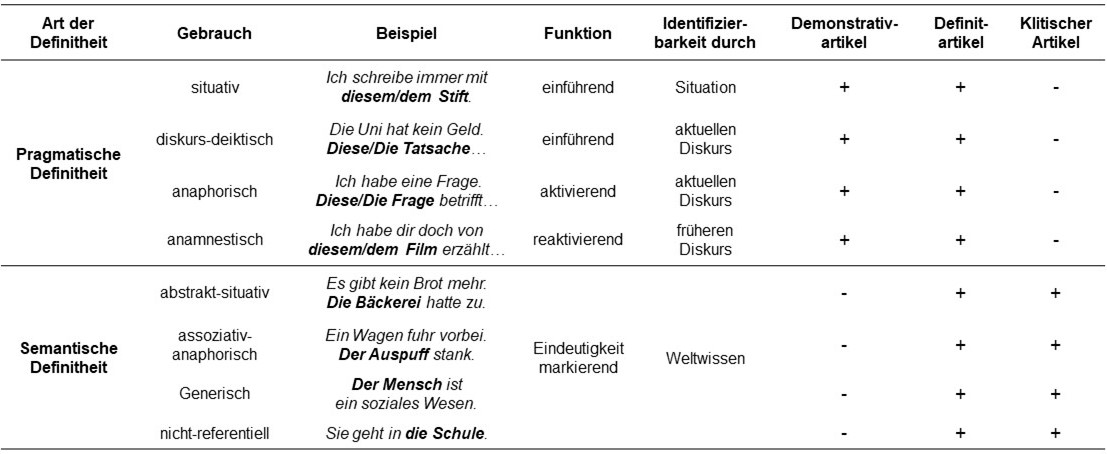
\includegraphics[width=\textwidth]{images/definit-kontexte-transparent.jpg}
\caption {Pragmatische und semantische Definita \is{Pragmatische Definita} \is{Semantische Definita} und ihre Gebrauchskontexte. (\textsc{dem}: Demonstrativartikel, \textsc{def}: Definitartikel, \textsc{klt}: Klitischer Artikel)\label{abb:definita}}
\begin{tabularx}{\textwidth}{>{\raggedright}p{\widthof{diskurs-deiktisch }}Q>{\centering}p{\widthof{reaktivierend}}cccc}
\lsptoprule
Gebrauch & Beispiel & Funktion & Identifizierbarkeit & \textsc{dem} & \textsc{def} & \textsc{klt}\\
         &          &          & durch \\\midrule                          
\multicolumn{7}{c}{Pragmatische Definitheit}\\\midrule
situativ & Ich schreibe immer mit \textit{diesem\slash dem Stift}. & einführend & Situation & + & + & \textminus\\
diskurs-deiktisch & Die Uni hat kein Geld. \textit{Diese\slash Die Tatsache}... & einführend & aktuellen Diskurs & + & + & \textminus\\
anaphorisch & Ich habe eine Frage. \textit{Diese\slash Die Frage} betrifft... & aktivierend & aktuellen Diskurs & + & + & \textminus\\
anamnestisch & Ich habe dir doch von \textit{diesem\slash dem Film} erzählt... & reaktivierend & früheren Diskurs & + & + & \textminus\\\midrule
\multicolumn{7}{c}{Semantische Definitheit}\\\midrule
abstrakt-situativ & Es gibt kein Brot mehr. \textit{Die Bäckerei} hatte zu. & Eindeutigkeit\newline markierend & Weltwissen & \textminus & + & +\\
assoziativ-anapho\-risch & Ein Wagen fuhr vorbei. \textit{Der Auspuff} stank. & Eindeutigkeit\newline markierend & Weltwissen & \textminus & + & +\\
generisch & \textit{Der Mensch} ist ein soziales Wesen. & Eindeutigkeit\newline markierend & Weltwissen & \textminus & + & +\\
nicht-referentiell & Sie geht in \textit{die Schule}. & Eindeutigkeit\newline markierend & Weltwissen & \textminus & + & +\\
\lspbottomrule
\end{tabularx}
\end{sidewaystable}

Die empirische Relevanz der semantischen \is{Semantische Definita} und \is{Pragmatische Definita} pragmatischen Definitheit\linebreak zeigt sich in Sprachen, die über zwei formal distinktive Artikelparadigmen verfügen -- bestehend aus einer unbetonten, reduzierten Form und einer betonten Vollform~-- die den beiden Definitheitsarten \is{Definitheit} entsprechen. Exemplarisch hierfür ist der von \textcite{Ebert1971} untersuchte  nordfriesische Dialekt Fering: Die phonologisch reduzierten A-Formen (\object{a/at}) sind den semantisch definiten Kontexten \is{Semantische Definita} vorbehalten, während die vollen D-Formen (\object{di/det/dön}) nur in pragmatisch-definiten Kontexten vorkommen \parencite[529]{deMulder2011}.\footnote{Eine Übersicht zu weiteren ähnlichen Artikelsystemen gibt \textcite[]{Studler2011}. Die semantischen Unterschiede von starken und schwachen Definita werden -- vor dem Hintergrund formaler Definitheitstheorien -- ausführlich in \textcite{Schwarz2009} diskutiert.}

\textcite[112--117]{Demske2001} nutzt die Löbnersche Distinktion, um die Artikeldistribution im Althochdeutschen zu untersuchen. Sie argumentiert dafür, dass ahd. \object{dër}  auf pragmatische Definitheitskontexte \is{Pragmatische Definita} beschränkt ist. Zur Illustration führt sie Belegstellen aus der ahd. Sprachperiode an, s. \xxref{ex:demske-prag1}{ex:demske-prag2}. 

\begin{exe} 
\ex \label{ex:demske-prag1}
	Situativer Gebrauch \\
	\gll ther thaz uuort gihorit \\
		der dieses Wort hört\\
	\trans \extrans{Der dieses Wort hört} (T 75.3)
\ex \label{ex:demske-prag2} 
	Anaphorischer Gebrauch \\
	\gll Ein búrg ist thar in lánte,...zi theru steti... \\
		eine Stadt ist dort im Land,...zu dieser Stadt...\\
	\trans  \extrans{Eine Stadt ist dort im Lande, ... zu dieser Stadt...} (O I, 11,23--26)
\end{exe}

\noindent 
Hingegen bleiben in den gleichen Texten funktionale Konzepte, also semantische \is{Semantische Definita} Definita \blockcquote[114]{Demske2001}{in der Regel} undeterminiert, s. \is{abstrakt-situativ} \REF{ex:demske-sem1} und \REF{ex:demske-sem2}. 

\begin{exe} 
\ex \label{ex:demske-sem1} 
	Abstrakt-situativer Gebrauch: Unika \is{Unikum} \\
	\gll Tho ward himil offan \\
		da ward Himmel offen \\
	\trans \extrans{Dann öffnete sich der Himmel} (O I,25,15)  
\ex \label{ex:demske-sem2} 
	Abstrakt-situativer Gebrauch: \is{Superlativ} Superlative \\
	\gll in ira bárm si sazta barno bézista \\
		 in ihren Schoß sie setzte Kind liebstes\\
	\trans  \extrans{Sie setzte das liebste Kind in ihren Schoß} (O I, 13,10)
\end{exe}

\noindent 
Die Belege suggerieren, dass das ahd. \object{dër} funktional dem heutigen \isi{Demonstrativartikel} gleicht. Zu einem solchen Schluss kommt auch \textcite{Philippi1997}, die neben Beispielen aus dem Althochdeutschen auch Belege aus dem  Altsächsischen und Gotischen anführt: \blockcquote[86]{Philippi1997}{The distribution of definite determiners in the older Gmc [Germanic, JF] languages seems to be very similar to the distribution of demonstrative pronouns in the
modern Gmc languages}. 

Interessanterweise lassen sich aber auch Belege finden, die diesem Befund entgegenstehen: Nach \textcite{Kraiss2012} gibt es bspw. schon im ahd. Isidor NPs \is{Nominalphrase (NP)} mit \object{dër} bei \is{Superlativ} Superlativkonstruktionen, z.B: \object{mit dhem hohistom salidhorn} \extrans{mit der höchsten Seligkeit} (I 5,9). Auch Unika kommen in einigen Fällen schon mit \object{dër} vor \parencite[75]{Szczepaniak2011a}, z.B. \object{ther himil} \extrans{der Himmel} (O I,11). Zum generischen \is{generisch} Gebrauch gibt es ebenfalls ganz unterschiedliche Beobachtungen. Kraiss geht nach seiner Durchsicht der größten althochdeutschen Textdenkmäler davon aus, dass weder im Isidor noch im Tatian generische \is{generisch} Phrasen \is{Phrase} mit \object{dër} vorkommen. Seinen Analysen nach wird diese Expansionsstufe \is{Expansion} erst bei Otfrid beschritten \parencite[133]{Kraiss2012}. \textcite[80]{Oubouzar1992} spürt determinierte generische \is{generisch} Referenzen allerdings schon im Tatian auf, s. \REF{ex:gen-tat-def}. Mit \object{ther man} liegt ein Fall von extensionaler Generizität  \is{generisch} vor; die Gattung Mensch wird verallgemeinert charakterisiert.  

\begin{exe} 
\ex \label{ex:gen-tat-def}
	\gll nio mag \textit{ther} \textit{man} iouuiht intphahen, noba imo iz gigeban uuerde fon himile \\
		nie mag der Mensch irgendetwas empfangen, {wenn nicht} ihm es gegeben werde von Himmel\\
	\trans \extrans{Der Mensch kann nichts empfangen, wenn es
ihm nicht vom Himmel geschenkt werde} (T 21,5)
\end{exe}
\noindent 
\textcite{Petrova2020} verweist auf einen ähnlichen Beleg, den bereits \textcite[60]{Hodler1954} in den Monseer Fragmenten beschreibt. Hier hat die Phrase \is{Phrase} \object{daer baum} eine  generische \is{generisch} Lesart:  \object{So auh fona des baumes obaze · arcennit · uuir(dit) daer · baum}, nhd. sinngemäß: \extrans{Den Baum erkennt man an seiner Frucht} (M 6,15). 

Ferner sind Präposition-Artikel-Klisen \is{Klitikon} ein weiteres wichtiges Indiz, dass \object{dër} bereits im Althochdeutschen in den Bereich der semantischen Definita \is{Semantische Definita} eindringt. Sie kommen bereits im Tatian, vor allem aber bei Otfrid vor \parencite[vgl.][]{Nubling1992,Schlachter2015}, z.B. \object{zemo seuue Galileę} \extrans{zum See von Galiläe} oder \object{zen jungoron} \extrans{zu den Jüngern} (O 3, 23,27). 

Die Beispiele verdeutlichen, dass Aussagen zur Semantik und \isi{Expansion} von \object{dër} nur schwer auf Basis von einzelnen, ausgewählten Belegstellen getroffen werden können. Um das Funk"-tions"-spektrum zu erfassen, muss erstens eine größere Menge an NPs \is{Nominalphrase (NP)} mit und ohne \object{dër} analysiert werden. Zweitens ist es notwendig, transparente Analysekriterien zu schaffen, die durch ein theoretisches Modell begründet sind. In der vorliegenden Arbeit ist dies die \citeauthor{Lobner1985}sche Unterscheidung in pragmatische \is{Pragmatische Definita} und semantische Definita \is{Semantische Definita} und damit zusammenhängend die oben genannten Gebrauchskontexte für Demonstrativ- \is{Demonstrativartikel} bzw. \isi{Definitartikel}. Die \isi{Operationalisierung} dieser Kriterien sowie die Auswahl der Belege wird im Methodenteil (Abschnitt \ref{sec:annotationsschritte}) erläutert. 

\section{Zusammenfassung}

In diesem Kapitel wurde das theoretische Gerüst vorgestellt, mit dem sich De"-mon"-stra"-tiv- \is{Demonstrativartikel} von Definitartikeln funktional unterscheiden lassen. Es ist deutlich geworden, dass ein bestimmtes Grammem (hier: das ahd. \object{dër}) nur dann als \isi{Definitartikel} klassifiziert werden kann, wenn es in semantisch-definiten Gebrauchskontexten \is{Semantische Definita} \parencite{Lobner1985} erscheint. Dies sind Fälle, in denen der Referent unabhängig von der Gesprächssituation eindeutig identifizierbar ist, was  sowohl beim abstrakt-situativen \is{abstrakt-situativ} (\object{Die Sonne scheint}) als auch beim assoziativ-anaphorischen \is{assoziativ-anaphorisch} Gebrauch (\object{Die Lehne an meinem Stuhl ist kaputt}) gegeben ist. Darüber hinaus wurden nicht-referentielle \is{Referentialität} Gebrauchskontexte diskutiert, darunter generische \is{generisch} Ausdrücke (\object{Der Mensch ist ein Säugetier}) und NPs \is{Nominalphrase (NP)} mit nicht-spezifischen \isi{Spezifizität} Referenten (\object{zur Kirche gehen}). Die Erkenntnisse aus der theoretischen Diskussion fließen in die Konzeption eines Annotationsleitfadens \is{Annotationsrichtlinien} ein (s. \ref{sec:annotationsschritte}). Es wird davon ausgegangen, dass die Gebrauchskontexte nicht immer klar zu unterscheiden sind. Ambige Fälle zwischen pragmatischen, d.h. situationsabhängigen, \is{Pragmatische Definita} und semantischen, also situationsunabhängigen \is{Semantische Definita} Gebrauchskontexten sind besonders relevant, da sie Brückenkontexte \isi{Brückenkontext} für den kategorialen Wandel sein können. 
